\documentclass[12pt,a4paper]{report}

%Set language
\usepackage[english]{babel}
\usepackage{enumerate}

% To import and adjust images
\usepackage{graphicx}
\usepackage[export]{adjustbox}
\usepackage[center]{caption}
\usepackage{subcaption}
\usepackage{float}
\usepackage{tabularx}

% To use monospaced font
\usepackage{courier}

% To build a clickable Toc
\usepackage{color} %May be necessary if you want to color links
\usepackage{hyperref}
\hypersetup{
    colorlinks=true, %set true if you want colored links
    linktoc=all,     %set to all if you want both sections and subsections linked
    linkcolor=black,  %choose some color if you want links to stand out
    urlcolor = black
}

%To load PoLitecnico's logo
\usepackage{titling}

% Command to hide subsections in the Toc
\setcounter{tocdepth}{1}

% I don't like dots in the Toc
\usepackage{tocloft}
\renewcommand{\cftdot}{}

%To improve the tables
\usepackage[table]{xcolor}

%To break line inside tables
%\usepackage[utf8]{inputenc}
%\usepackage{fourier} 
%\usepackage{array}
\usepackage{makecell}
%\renewcommand\theadalign{bc}
%\renewcommand\theadfont{\bfseries}
\renewcommand\theadgape{\Gape[4pt]}

% Path relative to the .tex file containing the \includegraphics command
\graphicspath{ {./images/} }

% To change the ToC title
\addto\captionsenglish{ \renewcommand {\contentsname} {Table of
contents}}

%logo
\pretitle{
	 \begin{center}
	 \LARGE
	 
\includegraphics[width = 0.6\textwidth]{logo}\\[\bigskipamount]
}
\posttitle{\end{center}}

% Here we go
\title{Artificial Neural Networks and Deep Learning \\ Homework 1 - Image Classification \\ \large version 1.0}
\author{Frantuma Elia, Fucci Tiziano}
\date{A.Y. 2020/2021}
\begin{document}
	\maketitle
	%Index
	\tableofcontents
	\chapter{Introduction}
		\section{Description of the task}
			The homework consists in an image classification problem on the proposed dataset. In particular, it is required to classify images depicting groups of people based on the number of masked people. In the specific, the solution must discriminate between images depending on the following cases:

\begin{enumerate} 
	\item all the people in the image are wearing a mask;
	\item no person in the image is wearing a mask;
	\item someone in the image is not wearing a mask.
\end{enumerate}
In the following 3 examples of image from the training belonging to the three cases.

Thus, the classification is performed on 3 different classes. Being a classification problem, given an image, the goal is to predict the correct class label.


			The RASD completely describes the system in terms of functional and nonfunctional requirements and
			serves as a contractual basis between the customer and the developer and it must be written in the language of
			the customer's domain of business/expertise, the DD's purpose instead is to provide a description for how the new
			system will be constructed, it provides a description of the system architecture, software, hardware, database
			design, and security.


			In particular this document will explain the following topics:
			\begin{itemize}
				\item high level architecture and its components' requirements;
				\item run-time behavior;
				\item design patterns;
				\item additional user interfaces information;
				\item implementation, integration and testing plan.
			\end{itemize}
		\section{Scope}
			Here a review of which is the scope of the application is made referring to what	has been stated in the RASD.


			SafeStreets is an application to be used both from civilians (users) and authorities, in order to help the latter and
			reduce traffic violations. Registered authorities can automatically receive reports made by users, so the service acts
			as an intermediary. 

		\section{Definitions, acronyms, abbreviations}
			\subsection{Definitions}
				\begin{itemize}
				\item \textbf{User}: a civilian customer that can use the application to:
					\begin{itemize}
					\item notify authorities of some violation;
					\item check which are the most dangerous (i.e. with the most violations) streets.
					\end{itemize}
				In this document, ``user", ``citizen" and ``civilian" are completely equivalent, where not specified.
				\item \textbf{Authority}: a member of the local police who has access to reports made by users. The
					authorities evaluate the reports sent by the user to determine if the violation stands.
				\item \textbf{Report}: a message consisting of:
					\begin{itemize}
					\item a picture showing the car in order to show the occurring violation;
					\item date and time of the picture;
					\item GPS position of the place where the violation occurred;
					\item the street where the violation occurred (automatically retrieved from the geographical position);
					\item the type of the violation (input by the user)
					\end{itemize}
				\item \textbf{Available}: a report is available for an authority if its position is within the municipality assigned
					to the authority.
				\item \textbf{Violation}: a situation that, according to the user who sent the report, is a violation of the
					traffic laws.
				\item \textbf{Intervention}: a brief text suggesting a possible solution in order to improve safety and
					discourage future violations.
				\end{itemize}
			\subsection{Acronyms}
				\begin{itemize}
				\item \textbf{AES}: \emph{Advanced Encryption Standard.}
				\item \textbf{API}: \emph{Application Programming Interface.}
				\item \textbf{DB}: \emph{Data Base.}			
				\item \textbf{DBMS}: \emph{Data Base Management System.}
				\item \textbf{DD}: \emph{Design Document.}
				\item \textbf{DMZ}: \emph{DeMilitarized Zone.}
				\item \textbf{GPS}: \emph{Global Positioning System.}
				\item \textbf{HTML}: \emph{HyperText Markup Language.}
				\item \textbf{ICM}: \emph{Item-Content Matrix.}
				\item \textbf{IEEE}: \emph{Institute of Electrical and Electronics Engineers.}
				\item \textbf{MVC}: \emph{Model-View-Controller.}
				\item \textbf{OCR}: \emph{Optical Character Recognition.}
				\item \textbf{PKC}: \emph{Public Key Cryptography.}
				\item \textbf{RASD}: \emph{Requirements Analysis and Specifications Document.}
				\item \textbf{RDBMS}: \emph{Relational Data Base Management System.}
				\item \textbf{REST}: \emph{REpresentational State Transfer.}
				\item \textbf{SHA-3}: \emph{Secure Hash Algorithm 3.}	
				\item \textbf{SS}: \emph{SafeStreets.}	
				\item \textbf{UI}: \emph{User Interface.}
				\item \textbf{UML}: \emph{Unified Modeling Language.}
				\item \textbf{UX}: \emph{User eXperience.}
				\item \textbf{XML}: \emph{eXtensible Markup Language.}
				\end{itemize}
		\section{Revision history}
			\begin{itemize}
				\item \textbf{Version 1.0}:
					\\ First release.
				\item \textbf{Version 1.1}:
				\begin{itemize}
					\item Improve class diagram;
					\item correct some typing errors;
					\item correct some errors in 2.4;
					\item other minor fixes.
				\end{itemize}
			\end {itemize}
		\section{Reference documents}
			The main reference documents are the ``SafeStreets Mandatory Project Assignment" specification document and the SafeStreets RASD. The complete list of references is provided in chapter 6.

		\section{Document structure}
			\begin{itemize}
				\item \textbf{Chapter 1} provides a brief explanation on the DD purpose and a quick introduction
					SafeStreets.
				\item \textbf{Chapter 2} aims to provide a description of the system's architecture.
				\item \textbf{Chapter 3} specifies the design of user interfaces and describes the user-application
					interaction.
				\item \textbf{Chapter 4} contains requirements traceability.
				\item \textbf{Chapter 5} describes the implementation plan.
				\item \textbf{Chapter 6} shows the effort of each group member.
				\item \textbf{Chapter 7} contains all the references used to make this document.
			\end{itemize}
	%end of first chapter

	\chapter{Architectural design}
		\section{Overview:	high-level	components	and	their	interaction}
	The application is built following the principles of the three-tier architecture: the three logic layers of presentation, 				application and data access rely on three corresponding hardware layers. This architecture is preferred to one-tier and 			two-tier architectures due to some important characteristics, some of which are:
	\begin{itemize}
	\item \emph{Flexibility}: each tier can be manged or scaled independently at any time, without affecting the others;
	\item \emph{Scalability}: following a scale-out approach, performances can be improved through node replication, without affecting the other tiers.
	Load balancing systems distribute the working load among the nodes;
	\item \emph{Maintainability}: because each tier is independent from the others, updates or changes can be released
	without affecting the whole system;
	\item \emph{Availability}: with this architecture, it is less likely to have failures that compromise the whole application.
	Load balancing and node replication minimize the performance loss when a failure occurs.
	\end{itemize}
	These aspects will be even better explained in section 2.6.
	A general view of the system architecture is provided in the following diagram, which provides an overview of the system architecture:
	\begin{figure}[H]
			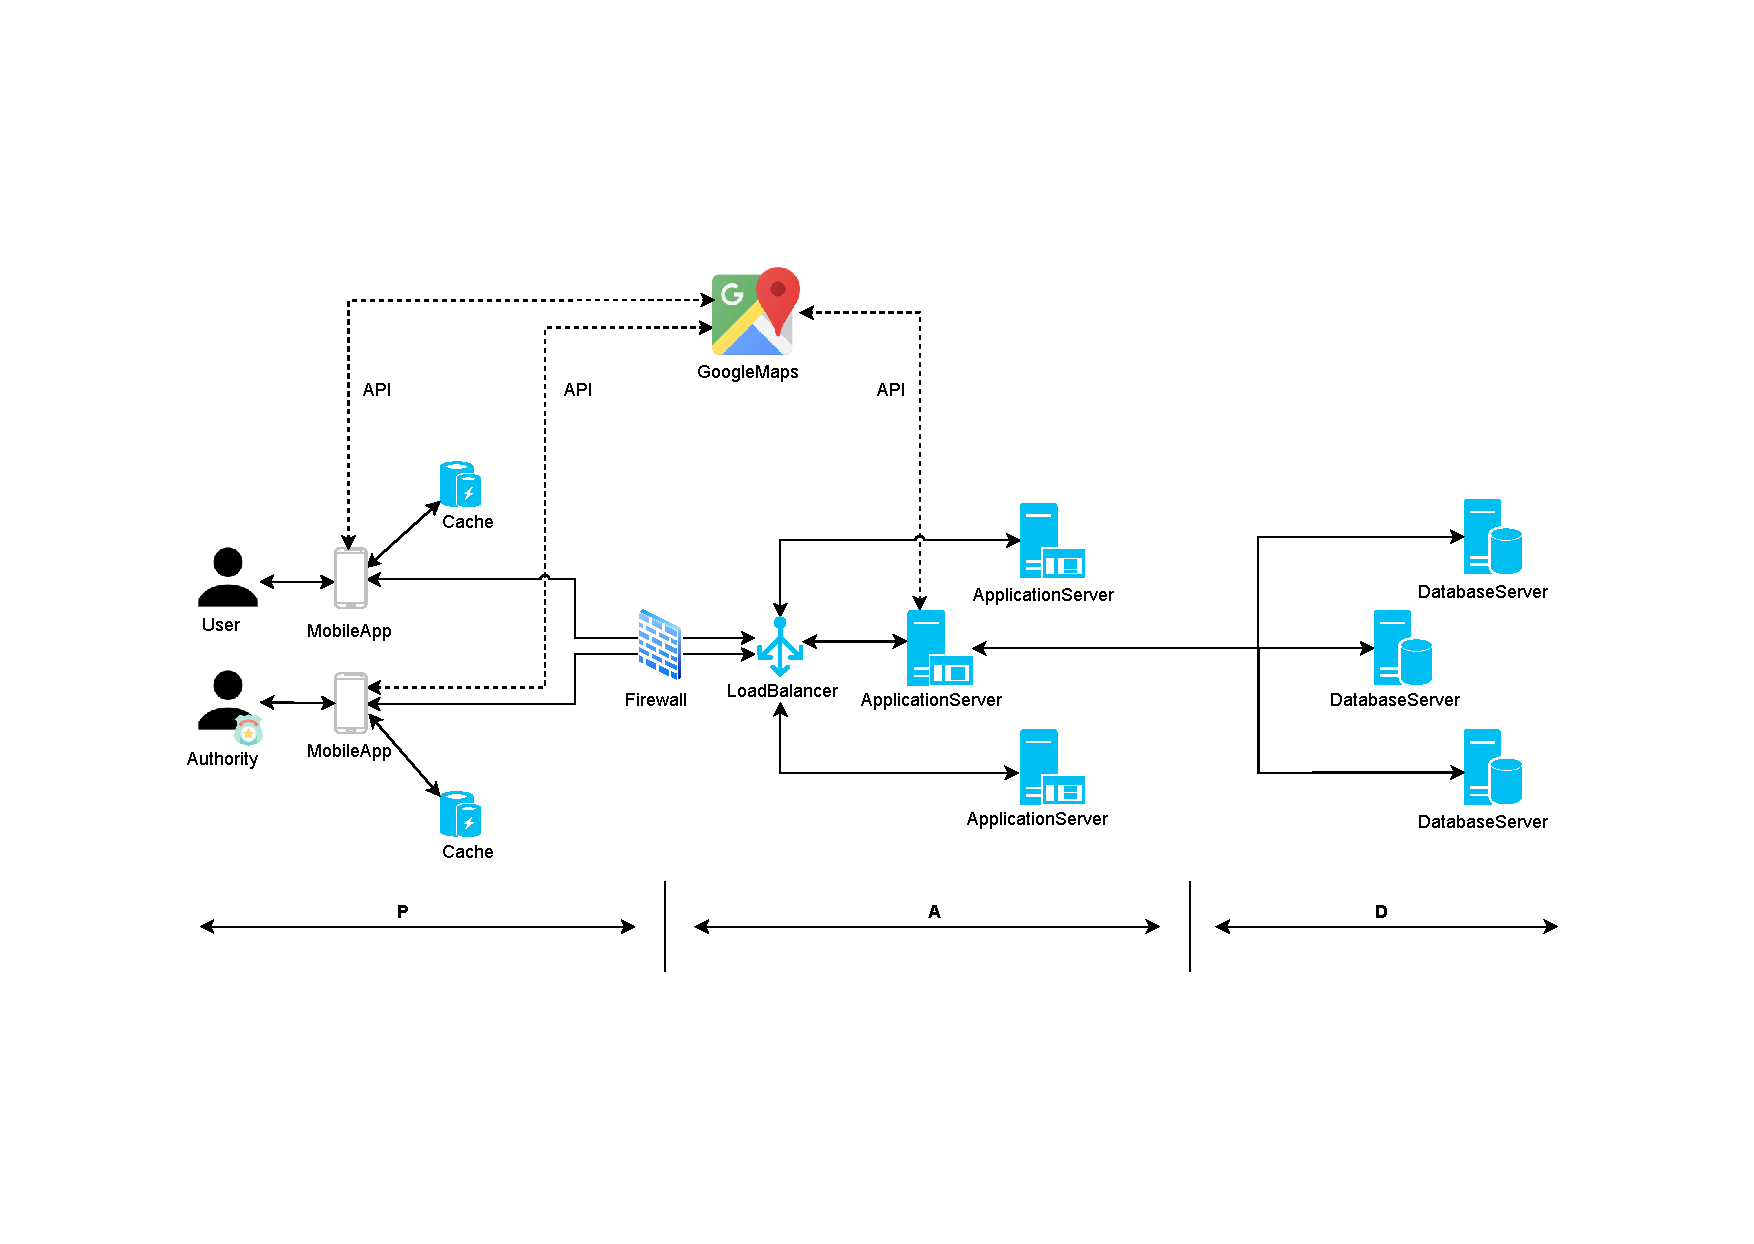
\includegraphics[scale = 0.6, center]{sysarch}
			\caption{System architecture}
	\end{figure}
	Users and authorities are provided with mobile devices and access the service through
	the SafeStreets mobile app. The mobile app communicates with the application layer, which
	is made by one or more application servers, linked to the database servers. The scale-out approach allows to adjust the number of hardware resources at any time. For what concerns the data access layer, database servers contain sensitive information, such as password hashes, license plate numbers, identification numbers and so on, so it is important to protect all the back-end of the application. In order to do this, the application and data access levels are protected by a firewall that performs traffic control at the level of the single packet, creating a DMZ in which the communication is safe. Another solution to reduce the computational load, as well as the messages, is the use of caches in the presentation tier: the mobile app stores on the mobile device memory part of the user's data, such as the sent reports and the results of reports evaluation, in order to make them available even when the users (or the authorities) have no access to Internet. This avoids many repeated requests for the same data, with heavy impact on the application and data access layers' performance.
The system also includes a recommender system: exploiting data mining techniques, such as association rules, it can suggest to the authorities of one municipality possible interventions to improve security on the streets.

		
	\chapter{Implementation, integration and test plan}
		\section{Implementation and test plan}
			To facilitate development, the system has been divided into subsystems, each of which corresponds to one of the
			above mentioned managers. They will be developed individually with a bottom-up approach and the order will be
			imposed by their importance to the system (how many sub-systems are depending from it) and for the customers.
			After the development of each subsystem, they will be tested to check their correctness and then
			some integration tests  will be executed. The system will use also some external systems, in particular Google Maps to have maps
			always updated and a DBMS to store all the data.
			\begin{table}[H]
				\rowcolors{2}{gray!25}{white}	
				\centering
				\begin{tabular}[width = \textwidth, position = center]{|c|c|c|}
					\hline
					{Subsystem} & {Importance for customers} & {Importance for development}\\
					\hline
					\hline
					Sign-up \& Login manager & Low & High\\
					\hline
					Report manager & High & High\\
					\hline
					Maps Manager & High & Low\\
					\hline
					History & High & Low\\
					\hline
					Evaluate & High & High\\
					\hline
					Suggestion & Medium & Medium\\
					\hline
					Notification Manager & Low & Low\\
					\hline
					Position Manager & Low & High\\
					\hline
				\end{tabular}
				\label{tab: }
			\end{table}
			\newpage
			It is important to stress that the reports and evaluation functionalities have to be developed and tested
			as a first step, because all the others functionalities rely on these two (except the functionalities for the suggestion
			about improving security on the streets).
			\begin{itemize}
				\item \textbf{Sign up \& login manager}: even if these two are not core functionalities of the system, they have a
					great importance in SafeStreets, because some functionality requires to keep trace in a unique way of
					who did what (for example history or suggestion); so this part has to be prioritized over the others
					(except ``Evaluate manager" and ``Report manager"). 
				\item \textbf{Report manager}: one of the core functionalities, it has to developed with maximum priority
					and tested as soon as possible, probably its more critic aspects are the OCR and the position. In order
					to be developed it needs a functioning ``Position manager", otherwise it will not be possible to convert
					the GPS position into a street name to understand where the traffic violation has been committed.
					Even if the ``Notification manager"  is in theory a sub-component of this, its development is not so
					crucial for the correct functioning of the system, so it can be developed in a second moment.  
				\item \textbf{Maps manager}: this component must be developed after the components necessary to
					ensure the creation and evaluation of reports (``Evaluate manager'' and ``Report manager'). It is not
					particularly important to choose the development order between the ``Map manager'' and ``History
					manager", the important thing is that they are properly developed and integrated before developing
					the others. This allow the use of the ``Visualize map" functionality, and seeing on the map the streets with
					most car accidents.
				\item \textbf{History manager}:  this component must be developed after the components necessary to
					ensure the creation and evaluation of reports (``Evaluate manager'' and ``Report manager'). It is not
					particularly important to choose the development order between the ``Map manager'' and ``History
					manager', the important thing is that they are properly developed and integrated before developing
					the other. This functionality allows the user to see the chronology of his reports.
				\item \textbf{Evaluate manager}: it is the second core functionality of the system. This functionality has to be
					able to correctly handle concurrency and various authorities that want to evaluate reports various
					reports at the same time. After the correct development of both the core functionalities an integration
					test is necessary to check the correct functioning of the complete system.  
				\item \textbf{Suggestion manager}: this is completely uncorrelated with the rest of the system, so it would be
					better to develop it as last thing, in this way the focus is on the core functionality of the system and
					the correct integration with the rest of the functionalities.
				\item \textbf{Position manager}: this component allows to get the road or location on the map of the
					user, it has the maximum priority, indeed it allows the system to understand where the report has been
					made.
				\item \textbf{Notification manager}: this component sends notifications to the users, it can be developed at
					last, on the top of the complete system because it is not a crucial aspect of the core functionalities.
			\end{itemize}
		\section{Integration}
		The following diagrams show which components will go through the process of 
			integration for a further clarification. The arrows starts from the component which ‘uses’ the other one.
			\subsection{Internal component}
				All the components are implemented and unit tested. Subsequently some components are 
				integrated and the integration is tested as well. 
				\newpage
				\begin{figure}[H]
						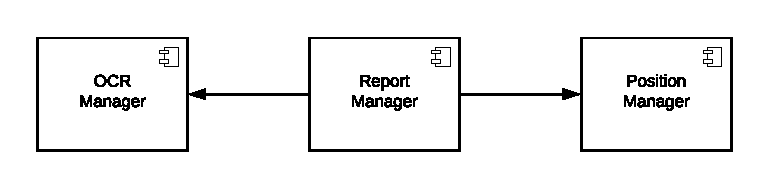
\includegraphics [center]{reportIntegration}
						%\caption{How reports are evaluated}
						\label{fig: interfaces}
				\end{figure}
				\begin{figure}[H]
						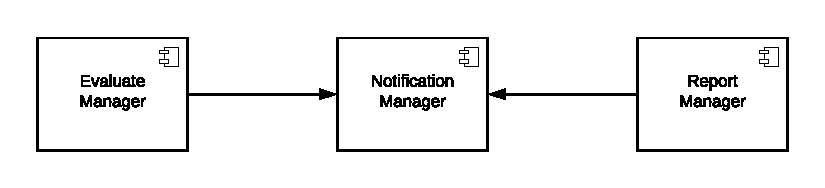
\includegraphics [center]{notificationIntegration}
						%\caption{How reports are evaluated}
						\label{fig: interfaces}
				\end{figure}
				\begin{figure}[H]
						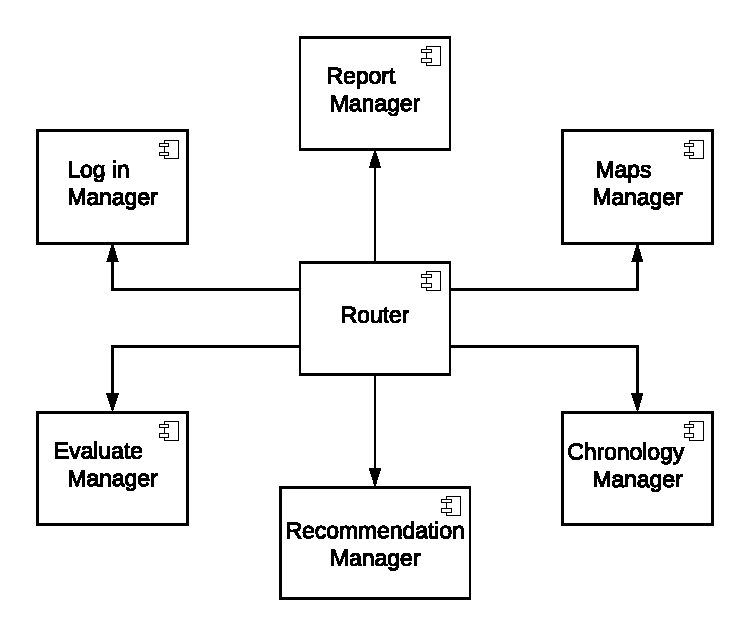
\includegraphics [center]{routerIntegration}
						%\caption{How reports are evaluated}
						\label{fig: interfaces}
				\end{figure}
				\begin{figure}[H]
						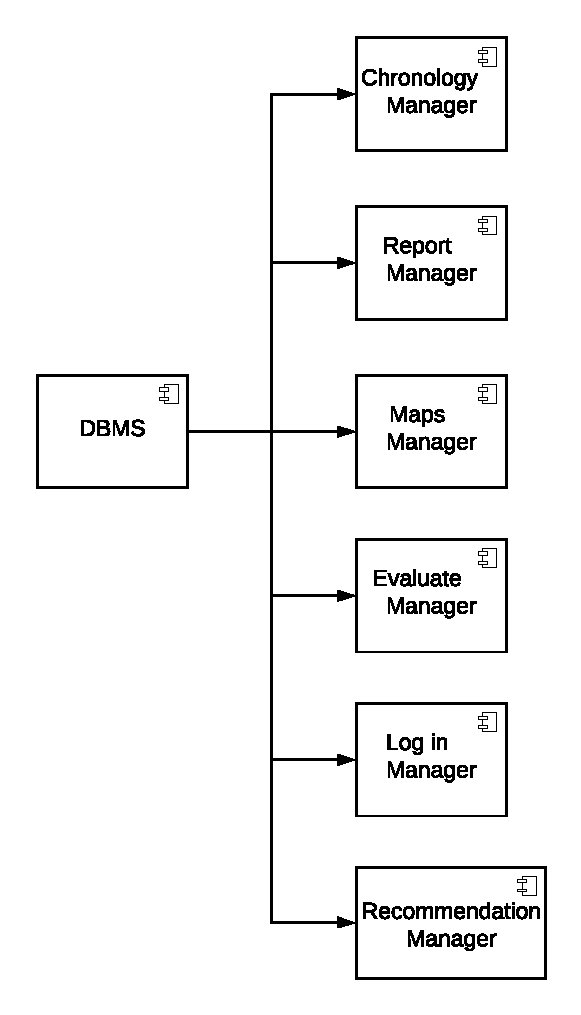
\includegraphics [center]{DBMS}
						%\caption{How reports are evaluated}
						\label{fig: interfaces}
				\end{figure}
				
			
	%end of fifth chapter

	\chapter{Effort spent}
		\begin{table}[H]
			\rowcolors{2}{gray!25}{white}
			\centering
			\begin{tabular}[width = \textwidth]{|c|c|c|}
				%\rowcolor{gray!50}
				\hline
				Chapter & Frangi (hours) & Fucci (hours)\\
				\hline
				\hline
				Chapter 1 & 1 & 0.5\\
				
				Chapter 2 & 13.5 & 17\\
				
				Chapter 3 & 1 & 2\\
				
				Chapter 4 & 2 & 4\\
				
				Chapter 5 & 8 & 1.5\\
				
				Total hours: & 25.5 & 25\\
				\hline
			\end{tabular}
			\label{tab: }
		\end{table}
	%end of sixth chapter
	\chapter{References}
		\section{Bibliography}
		\begin{itemize}
			\item Course slides from Software Engineering 2 - \emph{Professor Elisabetta Di Nitto};
			\item SafeStreets Requirement Analysis and Specification Document - \emph{Alberto Frangi, Tiziano Fucci};
			\item 1016-1987, IEEE Recommended Practice for Software Design Descriptions - \emph{IEEE}.
		\end{itemize}
		\section{Tools}	
		\begin{itemize}		
		\item StarUML 3.1.0 - to draw and export UML diagrams;
		\item \url{lucidchart.com} - to draw, share and export sequence diagrams;
		\item \url{draw.io} - to draw and export other diagrams;
		\item TeX Live 2019 - to write and organize this document;
		\item GitHub 2.23.0 - version control.
		\end{itemize}
	%end of seventh chapter
\end{document}
